\section{Strmentazione}
	In qest'esperienza esperienza sono state impiegate :
	\begin{itemize}
		\item 2 circiti integrati SN7400 usati per costituire i circuiti in esame
		\item varie resistenze e capacità impiegate anch'esse per il montaggio dei circiti
		\item 1 DIP switch a 4 interruttori
		\item 1 diodo 1N418
		\item 2 diodi LED, impiegati per rendere osservabile visivamente le tabelle di verità. 
		\item Il circito impulsatore basato sul Arduino nano montato nell'esperienza n:10
		\item un multimetro digitale
		\item un oscilloscopio digitale 
		\item un generatore di funzioni d'onda
	\end{itemize}
\section{verifica tabella NEND}
	Per la verifica della tabella di verità di nua porta NEND \tablename{ \ref{t:NEND}}
	\begin{table}[htb]
		\centering
		\begin{tabular}{sss}
				\toprule
				\text{ingresso} A & \text{ingresso} B &\text{uscita porta NAND }$\overline{A\cdot B}$	\\
				\midrule
				0  & 0 & 1\\
				0  & 1 & 1\\
				1  & 0 & 1\\
				1  & 1 & 0\\
				\bottomrule
			\end{tabular}
			\caption{Tabella di verità di una porta NEND.}
			\label{t:NEND}
		\end{table}
	si è procedto in due maniere distinte; una prima verifica visiva che impieghi il DIP switch in dotazione; ed una che impieghi il circito implsatore basato su ardino.
	Per entrambi i modi si è montato il circito in \figurename{ \ref{f:NEND}}.
	In tale circito si è 
	impiegata na resistenza di pll-ps $R_{1}=$\SI{0	\pm 4	}{\ohm} per migliorare 
	l'operatività del circito montato limitando la richiesta di corrente;
	il diodo LED D1 è posto in serie con $R_{1}$ e chiso sl GROND
	L'integrato  SN7400 è stato alimentato con na tensione di alimentazione $V_{cc}=$\SI{  0 \pm 4  }{\volt}.
	\begin{figure}[htb]
		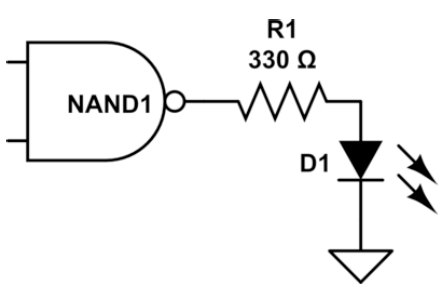
\includegraphics[scale=0.35]{../Figs-Tabs/NEND.png}
	\end{figure}\label{f:NEND}
\subsection{osservazione con dip switch}
	Essendo le delle porte NAND impiegate basate su logica TTL quando esse non risultino collegate a terra si ottiene in uscita un segnale corrispondente allo stato HIGH; cosa che non avviene qalora si abbia n collegamento a terra.
	Si è pertanto procedto a collegare gli ingressi 1 e 2 del deap switch alla tensione di GROND ed i piedini  3 e 4 rispettivamente agli ingressi A e B del NEND.
	
	Il diodo led  essendo acceso qalora l'scita del NEND sia alta
	e spento qalora  l'scita sia in stato LOW
	permette la verifica della tabella di verità.
	
	Si è procedto pertanto alla verifica della tabella di verità provando le varie permitazioni degli switch 1 e 2, ottenendo n perfetto accordo con \tablename{ \ref{t:NEND}}.
\subsection{Impiego di Ardino e del oscilloscopio}\label{sez:ard}
	Per effettare na lteriore verifica di tale tabella di verità 
	si è procedto a collegare le porte A e B della porta NOT rispettivamente alle 
	scite Y1 ed Y2 del circito implsatore realizzato con ardino nell'esperienza 10
	e collegata l'scita all'oscilloscopio.
	
	Essendo le traccie ottente alle porte Y1 e Y2 dell'implsatore de onde qadre 
	sfasate relativamente di $\pi/2$ s di n periodo generano ttte le permtazioni di de ingressi ad n bit.
	Si riportano le acqisizioni ottente dall'oscilloscopio
	\begin{figure}[hb]
		\centering
		\subfloat[acqsizione delle tensioni in ingresso nella porta NEND; A (ch1) ed B (ch2)]{
		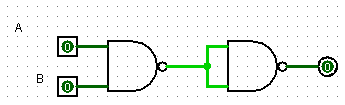
\includegraphics[scale=0.35]{../Figs-Tabs/ENd.png}
		\label{f:ing}
	}\\
	\subfloat[acqsizione scita porta NEND (ch1) ed tensione in ingresso B (ch2)]{
		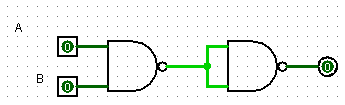
\includegraphics[scale=0.35]{../Figs-Tabs/ENd.png}
		\label{f:sci}
	}\\
	\caption{acqsizioni delle schermate impiegate per la verifica di \tablename{ \ref{t:NEND}}.}
	\label{f:osci}
\end{figure}.
	Per rendere significativa l' acqisizione dell'scita dalla porta NEND ( \figurename{ \ref{f:sci}} ) si è acqisita contemporaneamente no dei de ingressi, nella fattispecie B; dopodiché si sono acqisite entrambi i segnali  in ingresso (\figurename{ \ref{f:ing}} ) qale indicazione dello stato di ingresso.
	
	Dall'osservazione della \figurename{ \ref{f:osci}} si ottiene n lteriore verifica della \tablename{ \ref{t:NEND}}.
\section{Progettazione e verifica semplici circiti logici}
	Per verificare le tabelle di verità dei segenti circiti si è impiegato il circito implsatore; ed in particolare la tecnica descritta in\textbf{ sezione \ref{sez:ard} };
	Si segnala che per ttta la zezione faremo riferimento alla \figurename{ \ref{f:ing}} qale riferimento.
	\subsection{AND}
	Per verificare l'andamento di n circito AND, essendo
	$$AND(A,B) = A \cdot B = \overline{(\overline{A \cdot B})}$$
	si è montato il circito in \figurename{ \ref{f:AND}} 
	\begin{figure}[htb]
		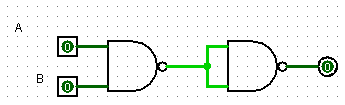
\includegraphics[scale=1.0]{../Figs-Tabs/ENd.png}
		\caption{rappresentazione di n circito AND realizzato con porte NAND. A e B rappresentano gli ingressi mentre si campiona in scita sl terzo terminale.}
	\end{figure}\label{f:AND}
.
	Tale circito presenta la tabella di verità riportata in \tablename{ \ref{t:AND}} 
	\begin{table}[htb]
		\centering
		\begin{tabular}{sss}
			\toprule
			\text{ingresso} A & \text{ingresso} B &\text{uscita porta AND }$A\cdot B$	\\
			\midrule
			0  & 0 & 0\\
			0  & 1 & 0\\
			1  & 0 & 0\\
			1  & 1 & 1\\
			\bottomrule
		\end{tabular}
		\caption{Tabella di verità di una porta AND.}
		\label{t:AND}
	\end{table}.
	la qale rislata a sa volta verificata dall'andamento osservato
	e riportato in \figurename{ \ref{f:osci-and}}
	
	\begin{figure}[hb]
		\centering
		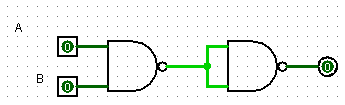
\includegraphics[scale=0.35]{../Figs-Tabs/ENd.png}
		\caption{acqsizione della schermata impiegate per la verifica di \tablename{ \ref{t:AND}}.
		scita porta AND (ch1) ed tensione in ingresso in B (ch2).
		}
		\label{f:osci-and}
	\end{figure}.
	\subsection{OR}
			Per la fnzione OR essendo $$ OR(A,B) = A + B = \overline{\overline{(A +B)}}= \overline{(\overline{A} \cdot \overline{B})}$$
			è stato montato il circito in \figurename{ \ref{f:OR}} 
		\begin{figure}[htb]
			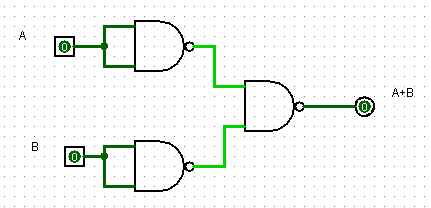
\includegraphics[scale=1.0]{../Figs-Tabs/OR.png}
			\caption{rappresentazione di n circito OR realizzato con porte NAND. A e B rappresentano gli ingressi mentre si campiona in scita sl terzo terminale.}
		\end{figure}\label{f:OR}.
		Tale circito presenta la tabella di verità riportata in \tablename{ \ref{t:AND}} 
		\begin{table}[htb]
			\centering
			\begin{tabular}{sss}
				\toprule
				\text{ingresso} A & \text{ingresso} B &\text{uscita porta AND }$A\cdot B$	\\
				\midrule
				0  & 0 & 0\\
				0  & 1 & 1\\
				1  & 0 & 1\\
				1  & 1 & 1\\
				\bottomrule
			\end{tabular}
			\caption{Tabella di verità di un circito OR.}
			\label{t:OR}
		\end{table}.
		la qale rislata a sa volta verificata dall'andamento osservato
		e riportato in \figurename{ \ref{f:osci-or}}
		
		\begin{figure}[hb]
			\centering
			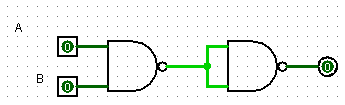
\includegraphics[scale=0.35]{../Figs-Tabs/ENd.png}
			\caption{acqsizione della schermata impiegate per la verifica di \tablename{ \ref{t:OR}}.
				scita circito OR (ch1) e tensione in ingresso in B (ch2).
			}
			\label{f:osci-or}
		\end{figure}.
	\subsection{XOR}
	Per la fnzione XOR essendo $$ XOR(A,B) = A \oplus B = (A \cdot \overline{B}) + (\overline{A} \cdot B) =
	 \overline{
	 	\overline{
	 		( A \cdot \overline{
	 			(A \cdot B) )
 			}	\cdot 
 		\overline{
 			(B \cdot \overline{
 				(A \cdot B)
 			} )
 		}
 	}
	}$$
	è stato montato il circito in \figurename{ \ref{f:XOR}} 
	\begin{figure}[htb]
		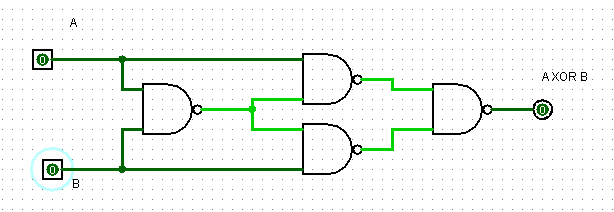
\includegraphics[scale=1.0]{../Figs-Tabs/XOR.png}
		\caption{rappresentazione di n circito XOR realizzato con porte NAND. A e B rappresentano gli ingressi mentre si campiona in scita sl terzo terminale.}
	\end{figure}\label{f:XOR}.
	Tale circito presenta la tabella di verità riportata in \tablename{ \ref{t:AND}} 
	\begin{table}[htb]
		\centering
		\begin{tabular}{sss}
			\toprule
			\text{ingresso} A & \text{ingresso} B &\text{uscita porta XOR }$A \oplus B$	\\
			\midrule
			0  & 0 & 0\\
			0  & 1 & 1\\
			1  & 0 & 1\\
			1  & 1 & 0\\
			\bottomrule
		\end{tabular}
		\caption{Tabella di verità di un circito XOR.}
		\label{t:XOR}
	\end{table}.
	la qale rislata a sa volta verificata dall'andamento osservato
	e riportato in \figurename{ \ref{f:osci-xor}}
	
	\begin{figure}[hb]
		\centering
		\includegraphics[scale=0.35]{../Figs-Tabs/NEnd.png}
		\caption{acqsizione della schermata impiegate per la verifica di \tablename{ \ref{t:XOR}}.
			scita circito XOR (ch1) e tensione in ingresso in B (ch2).
		}
		\label{f:osci-xor}
	\end{figure}.
\subsection{Circito sommatore ad n bit}	
	Per realizzare il circito sommatore richiesto abbiamo assnto
	che esso potesse costitirsi s n scita [scita 1] di na fnzione XOR, per esprimere il bit più significativo;
	ed da na fnzione AND sll scita rimanente [scita 2] per esprimere il meno significativo.
	Si è montato pertantonto il circito in \figurename{ \ref{f:somma}} 
		\begin{figure}[htb]
		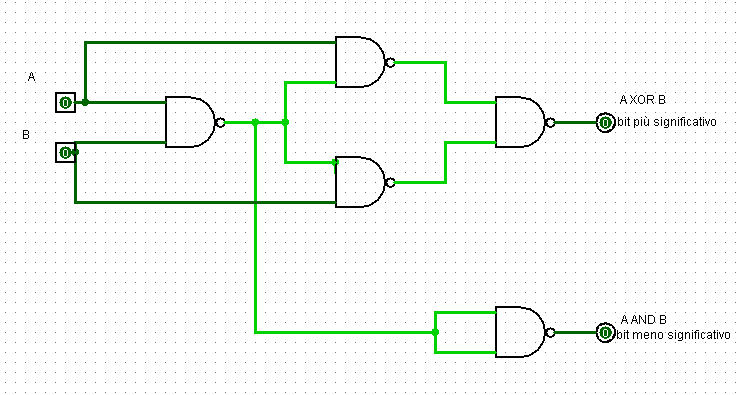
\includegraphics[scale=1.0]{../Figs-Tabs/somma.png}
		\caption{rappresentazione di n circito sommatore a 2 ingressi e 2 scite.}
	\end{figure}\label{f:somma}
	.
	L'andamento del circito rislta verificato dalla 
	
	\begin{figure}[hb]
	\centering
	\subfloat[acqsizione della tensione in scita dal circito XOR (ch1) ed in ingresso B (ch2);
	tale figra costitisce insieme alla \figurename{ \ref{f:ing}} n riferimento]{
		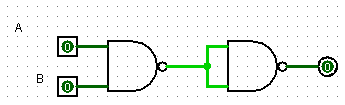
\includegraphics[scale=0.35]{../Figs-Tabs/ENd.png}
		\label{f:ing-somma}
	}\\
	\subfloat[acqsizione delle tensioni in scita dal circito XOR (ch1) ed in scita dal circito AND (ch2)]{
		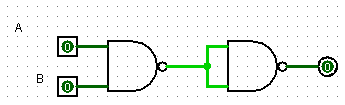
\includegraphics[scale=0.35]{../Figs-Tabs/ENd.png}
		\label{f:sci-somma}
	}\\
	\caption{acqsizioni delle schermate impiegate per la verifica del fnzionamento del circito sommatore.}
	\label{f:osci-somma}
\end{figure}
	\figurename{ \ref{f:osci-somma}}.
	Si pò infatti osservare che l'scita assma alternativamente i valori $00-01-10-11$.
\section{Mltivibratore MONOSTABILE}